\begin{figure}[t!]

  \setlength{\unitlength}{\textwidth}

  \begin{picture}(1,0.35)(0,0.725)

    \put(-0.01,0.76){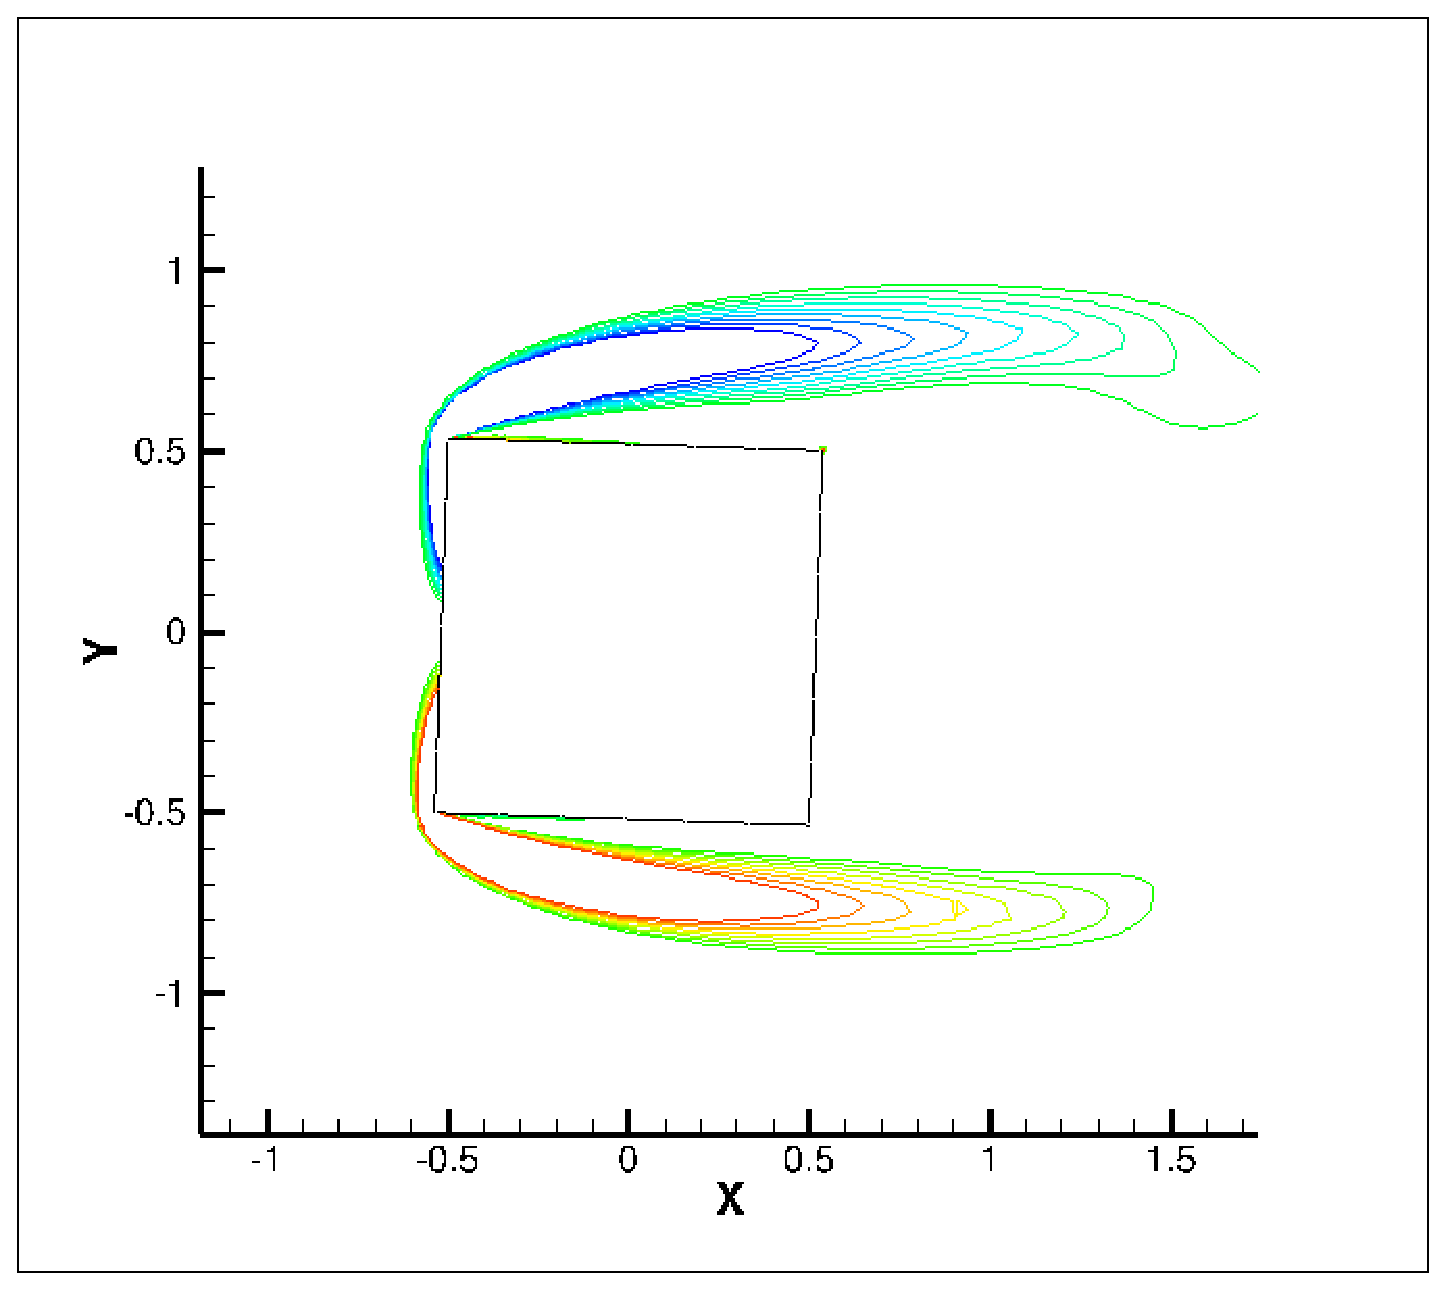
\includegraphics[width=0.33\unitlength]{./chapter-literature-revirw/fnp/square-2.eps}}
    \put(0.335,0.76){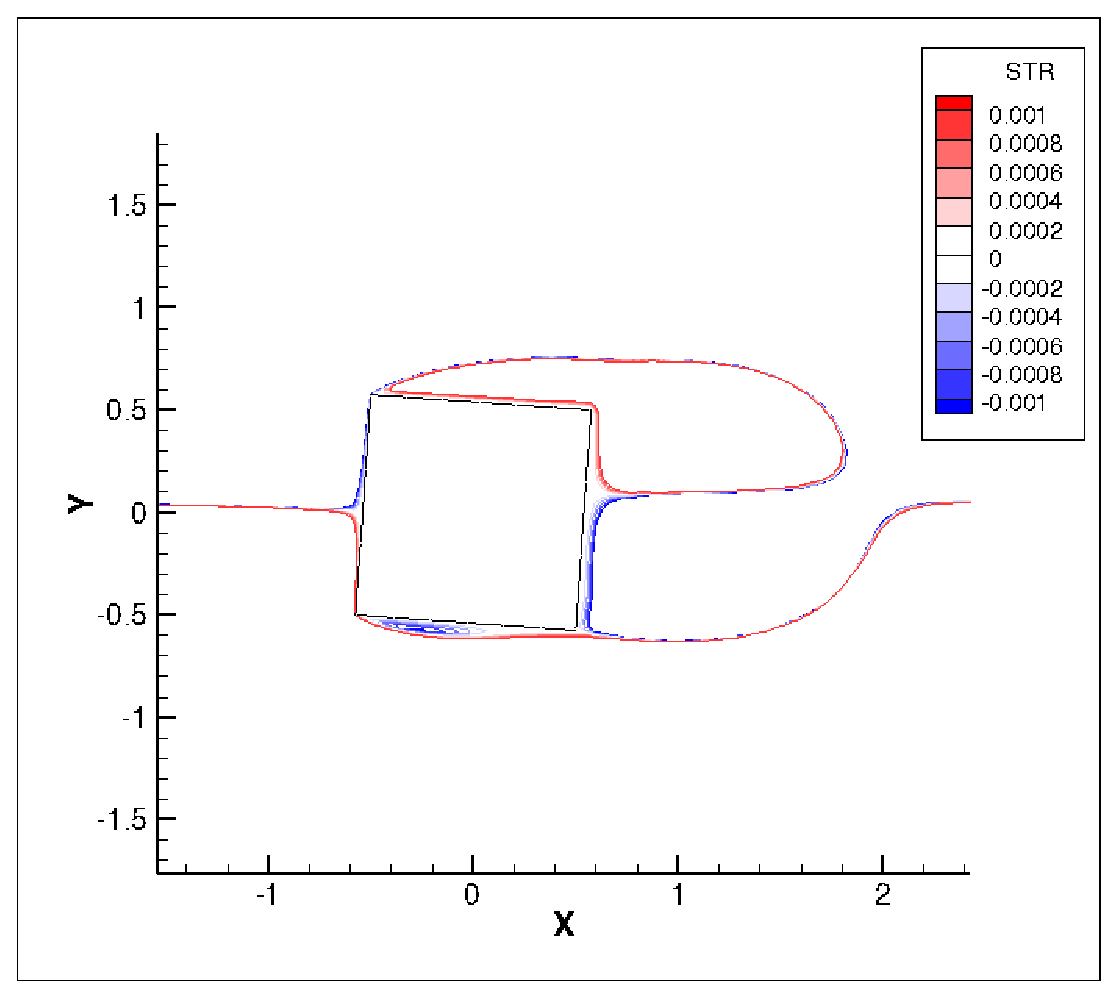
\includegraphics[width=0.33\unitlength]{./chapter-literature-revirw/fnp/square-4.eps}}
    \put(0.68,0.76){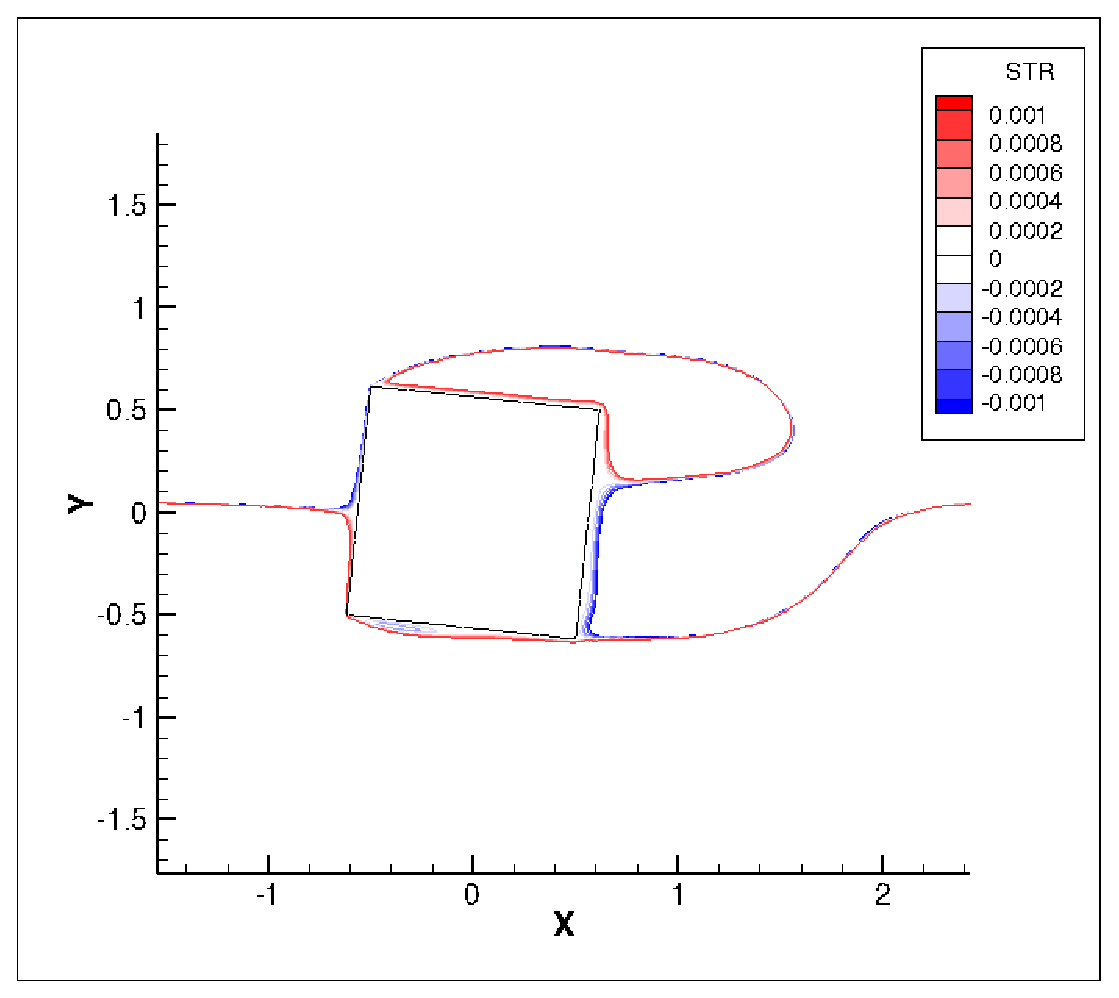
\includegraphics[width=0.33\unitlength]{.//chapter-literature-revirw/fnp/square-6.eps}}

   
    
    \put(0.0,0.735){(a)}    
    \put(0.34,0.735){(b)}
    \put(0.685,0.735){(c)}
  
  \end{picture}

  \caption{Vorticity contours of time averaged flow field on a stationary square section at $\reynoldsnumber=200$ at different incidence angles. (a) $2^{\circ}$ ($C_{y}$ increases),(b) $4^{\circ}$ ($C_{y}$ peaks) and (c) $2^{\circ}$ ($C_{y}$ decreases). The bottom shear layer comes closer to the bottom wall and reattaches as the angle of incidence increases.}
  \label{fig:shear_layers}
\end{figure}




